\documentclass{ResumeDesignFormat1}
\usepackage[english]{babel}
\usepackage{marginnote}
\usepackage{tikz}
\usepackage{hyperref}
\usetikzlibrary{positioning}
\usetikzlibrary{backgrounds}
\usepackage{tkz-berge}
\usepackage{sectsty}
\sectionfont{\footnotesize}
\subsectionfont{\Large}
\subsubsectionfont{\large}
\paragraphfont{\lfootnotesize}
\usepackage{pagecolor}
\definecolor{c1}{rgb}{0.858, 0.188, 0.478}
\definecolor{c2}{RGB}{219, 48, 122}
\definecolor{c3}{cmyk}{0, 0.7808, 0.4429, 0.1412}
\definecolor{c4}{gray}{0.1}
\definecolor{c5}{RGB}{142, 68, 173}
\definecolor{blueish}{rgb}{0.565,0.886,1} 
\definecolor{greenish}{rgb}{0.565,1,0.886}
\definecolor{darkgray}{rgb}{0.15,0.15,0.15} 
\definecolor{lightgray}{rgb}{0.6,0.6,0.6}
\graphicspath{{Figures/1/}}

\begin{document}
%-----------------------------------------------------------------------------------------------------------------------------------------%
%---------------------------------------Figure 1------------------------------------------------------------------------------------------% 
%-----------------------------------------------------------------------------------------------------------------------------------------%

%-----------------------------------------------------------------------------------------------------------------------------------------%
%---------------------------------------Line Graph ---------------------------------------------------------------------------------------%
%-----------------------------------------------------------------------------------------------------------------------------------------%
\centering
\vspace{12pt}
\begin{figure}[ht]
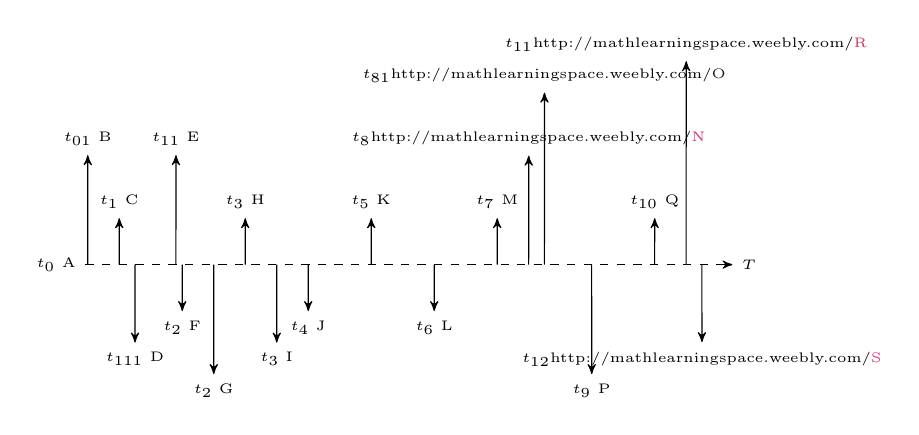
\begin{tikzpicture}[->,>=stealth',scale=0.4]
%-----------------------------------------------------------------------------------------------------------------------------------------%
\node(T0) at (16,0) {\tiny $t_{0}$ A};
\node(T01) at (17,4) {\tiny $t_{01}$ B};
\node(T1) at (18,2) {\tiny $t_{1}$ C};
\node(T111) at (18.5,-3) {\tiny $t_{111}$ D};
\node(T11) at (19.8,4) {\tiny $t_{11}$ E};
\node(T2) at (20,-2) {\tiny $t_{2}$ F};
\node(T21)  at (21,-4) {\tiny $t_{2}$ G};
\node(T3) at (22,2) {\tiny $t_{3}$ H};
\node(T31) at (23,-3) {\tiny $t_{3}$ I};
\node(T4) at (24,-2) {\tiny $t_{4}$ J};
\node(T5) at (26,2) {\tiny $t_{5}$ K};
\node(T6) at (28,-2) {\tiny $t_{6}$ L};
\node(T7) at (30,2) {\tiny $t_{7}$ M};
\node(T8) at (31,4) {\tiny $t_{8}$\href{http://mathlearningspace.weebly.com/}{\textcolor{c1} {N}}};
\node(T81) at (31.5,6) {\tiny $t_{81}$\href{http://mathlearningspace.weebly.com/}{\textcolor{c4} {O}}};
\node(T9) at (33,-4) {\tiny $t_{9}$ P};
\node(T10) at (35,2) {\tiny $t_{10}$ Q};
\node(T101) at (36,7) {\tiny $t_{11}$\href{http://mathlearningspace.weebly.com/}{\textcolor{c3} {R}}};
\node(T102) at (36.5,-3) {\tiny $t_{12}$\href{http://mathlearningspace.weebly.com/}{\textcolor{c2} {S}}};
\node(T) at (38,0) {\tiny $T$};
%---------------------------------------------------------------------------------------------------------------------------------------------------------%
\draw[->,thin, dashed] (T0)--(T);
\draw [->,thin] ( 17,0) -- (T01);
\draw [->,thin] ( 18,0) -- (T1);
\draw [->,thin] ( 18.5,0) -- (T111);
\draw [->,thin] ( 19.8,0) -- (T11);
\draw [->,thin] ( 20,0) -- (T2);
\draw [->,thin] ( 21,0) -- (T21);
\draw [->,thin] ( 22,0) -- (T3);
\draw [->,thin] ( 23,0) -- (T31);
\draw [->,thin] ( 24,0) -- (T4);
\draw [->,thin] ( 26,0) -- (T5);
\draw [->,thin] ( 28,0) -- (T6);
\draw [->,thin] ( 30,0) -- (T7);
\draw [->,thin] ( 31,0) -- (T8);
\draw [->,thin] ( 31.5,0) -- (T81);
\draw [->,thin] ( 33,0) -- (T9);
\draw [->,thin] ( 35,0) -- (T10);
\draw [->,thin] ( 36,0) -- (T101);
\draw [->,thin] ( 36.5,0) -- (T102);
\end{tikzpicture}
\caption{\footnotesize TMLS - The Mathematical Learning Space}
\end{figure}
%-----------------------------------------------------------------------------------------------------------------------------------------%
%----------------------------Summary of Experience Examples-------------------------------------------------------------------------------%
%-----------------------------------------------------------------------------------------------------------------------------------------%
\begin{enumerate}
\item {Weebly}{\href{http://mathlearningspace.weebly.com/}{\textcolor{c5}{Math Learning Space-Weebly}}}
\item {GitHub}{\href{https://github.com/MathematicalLearningSpace}{\textcolor{c5}{Mathematical Learning Space-GitHub}}}
\end{enumerate}
%-----------------------------------------------------------------------------------------------------------------------------------------%
%----------------------------Summary of Experience Table----------------------------------------------------------------------------------%
%-----------------------------------------------------------------------------------------------------------------------------------------%
\begin{table}[H]\centering
\tiny
\begin{tabular}{p{1cm}p{4cm}p{3cm}p{2cm}p{2cm}p{2cm}}
Job ID & Title & Location & Accomplishments & Start Date & End Date \\
\hline
1 & & & & & \\
\hline
\end{tabular}
\end{table}

%-----------------------------------------------------------------------------------------------------------------------------------------%
%---------------------------------------Lecture Posters, Music Compositions and Articles--------------------------------------------------%
%-----------------------------------------------------------------------------------------------------------------------------------------%
\begin{enumerate}
\item Lecture Poster 1
\end{enumerate}

%------------------------------------------------------------------------------------------------------------------------------------------%
%---------------------------------------Graphics Design Portfolio:Article 1 Example--------------------------------------------------------%
%------------------------------------------------------------------------------------------------------------------------------------------%
\footnotesize
\begin{figure}[h]
	\centering
	\begin{minipage}[b]{0.5\linewidth}
		\includegraphics[scale=0.25]{Example_1_Figure_0.png}
		\caption{\footnotesize Example 1 }
		\label{fig:FigureA}
	\end{minipage}\hfill
	\begin{minipage}[b]{0.5\linewidth}
		\includegraphics[scale=0.25]{Example_1_Figure_0A.png}
		\caption{\footnotesize Example 2}
		\label{fig:FigureB}
	\end{minipage}\hfill
	\begin{minipage}[b]{0.5\linewidth}
		\includegraphics[scale=0.25]{Example_1_Figure_0B.png}
		\caption{\footnotesize Example 3}
		\label{fig:FigureC}
	\end{minipage}\hfill
	\begin{minipage}[b]{0.5\linewidth}
		\includegraphics[scale=0.25]{Example_1_Figure_0C.png}
		\caption{\footnotesize Example 4}
		\label{fig:FigureD}
	\end{minipage}\hfill
	\caption{\textcolor{c5}{\textbf{Classroom Lecture Model Series 1:}}\footnotesize Example 1 }
	\label{fig:Figure1}
\end{figure}

\end{document}
